%---------------------------
%	PREAMBLE
%---------------------------

\documentclass{article}

\usepackage[english]{babel}
\usepackage[utf8]{inputenc}
\usepackage{fourier}
\usepackage{fancyhdr}
\usepackage[parfill]{parskip}
\usepackage{hyperref}
\usepackage{graphicx}
\usepackage{float}
\usepackage{listings}
\usepackage{fourier}
\usepackage{tikz}
\usetikzlibrary{shapes.geometric, arrows}
\usepackage{textcomp}

\newcommand{\forceindent}{\leavevmode{\parindent=2em\indent}}

%------------------------%------------------------%

\begin{document}

\pagestyle{fancy}
\fancyhf{}
\rhead{Doing Survey Research \the\year}
\lhead{https://github.com/Yuji-Shimohira-Calvo/DSR}
\rfoot{Page \thepage}

\section*{\hfil Lab Worksheet V \hfil}
\subsection*{Bivariate analysis}

Today you will learn how to examine the empirical relationship between two variables in Stata. This examination can be both \textit{descriptive} and \textit{inferential}. There is a number of different ways by which you can achieve this, for instance, cross-tabulations, scatterplots, correlation coefficients, and linear regression. However, whether bivariate analysis is descriptive or inferential will ultimately depend on two things: one is the level of measurement of your variables, and the other is whether you can consider one variable ``\textit{dependent}'' and the other ``\textit{independent}.'' In this exercise we are going to work with categorical variables in the \textbf{essuk12v3.dta} dataset which you can download from LEARN (please mind the ``v3'' in the dataset's name).

\begin{figure}[H]
	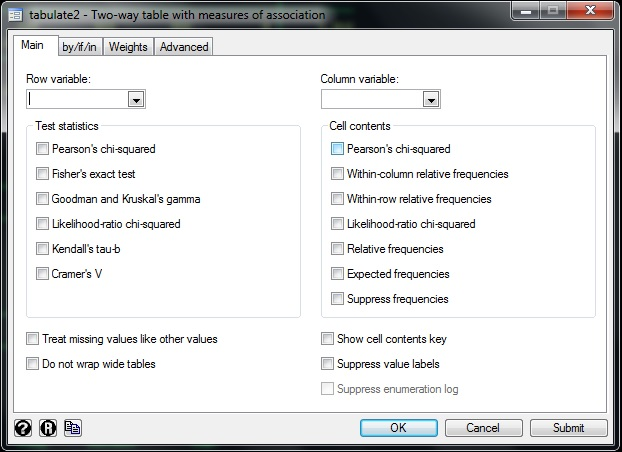
\includegraphics[width=\linewidth]{../img/tabulate2.jpg}
	\caption{Two-way table with measures of association.}
\end{figure}

\subsubsection*{Cross-tabulations}

A \textit{cross-tabulation} is a table with rows and columns in which categorical variables (their frequencies) are represented. These tables are also called ``\textit{contingency tables}'' because the category of a case in one variable is \textit{contingent} on its category in the other variable. For example, the political party a person supports may be contingent on their socio-economic status. If you can identify dependent and independent variables, it is customary to place your dependent variable in columns and your independent variable in rows. Let’s start with a cross-tabulation of whether a person has ever been member of a trade union and their gender. In this example, we are going to assume that whether a person has ever been member of a trade union is more likely if the person is a man (remember that assumptions are given by social theory; numbers are useless without theory!). Here ``gender'' is our independent variable and ``trade union membership'' is our dependent variable.

To get a cross-tabulation of the variables ``gender'' and ``trade union membership'' we can use the command \texttt{tabulate}, but this time we are going to feed in two variables. Alternatively, you can use Stata's menu: go to \textit{Statistics} > \textit{Summaries, tables, and tests} > \textit{Frequency tables} > \textit{Two-way table with measures of association}. You should now see something like Figure 1 above. Select ``gender'' as your \textit{Row variable} and ``union'' as your \textit{Column variable}.Under \textit{Cell contents} tick \textit{Within-row relative frequencies}, this will give you percentages that add up to 100 percent for each row.

\begin{figure}[H]
	\centering
	\resizebox{0.65\textwidth}{!}{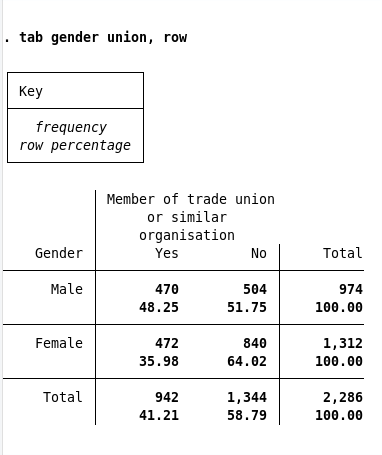
\includegraphics{../img/tab_gender_union_row.png}}
	\caption{Cross-tabulation of gender and union membership.}
\end{figure}

Remember that \texttt{tabulate} can be shortened to \texttt{tab}. The column on the right provides you with the total for each row. The first numbers in each cell of the table are frequencies, whereas the numbers below are percentages. As you can see in Figure 2, there are 974 males in total, 470 of them have ever been member of a trade union. On the other hand, there are 1,312 females in total and 472 of them have ever been member of a trade union. Because each row (i.e., each category of ``gender'') has a different number of observations, it is not easy to compare \textit{absolute frequencies}. It appears that more females have ever been in a trade union, however this is not true when we look at it in \textit{relative terms}. Percentages are greatly useful in cases like this one: in absolute terms, this dataset shows more females that have ever been member of a trade union, but when taking into consideration the number of males and females, it appears that more males, in relative terms, have ever been member of a trade union (48.25 percent versus 35.98 percent). Another important thing to keep in mind is the ``direction'' of the percentages; in this example the proportions have been computed in rows (horizontally), thus you should carry your comparison in columns (vertically).

\subsubsection*{Chi-squared test ($\chi^2$)}

The difference between men and women who have ever been member of a trade union is not very big, but it might be considerable (remember, 48.25 percent versus 35.98 percent). Did we get this difference by \textit{chance}? The sample you are working with is pretty big (2,286 cases), so you may think that there is no reason to think that the difference between men and women is given by chance. Nevertheless, it is good practice to check whether it is \textit{statistically significant}. We can use the chi-squared statistic ($\chi^2$) for examining the likelihood that your results occurred by chance. In simple words, the logic of this test is that if it is extremely unlikely to get this difference between men and women, with such a big sample size, then you can be confident that there was a real difference. However, do not confuse this with the researcher's call to assess whether the difference between men and women is substantially (i.e., theoretically) important.

To perform a chi-squared test in Stata you can use the menu shown in Figure 1, but this time tick \textit{Person's chi-squared} under \textit{Test statistics} and, additionally, you can also tick \textit{Expected frequencies} under \textit{Cell contents}. Alternatively, you can use the following command:

\begin{lstlisting}
tabulate gender union, row chi2 expected
\end{lstlisting}

The option \texttt{row} gives you percentages in rows, whereas \texttt{chi2} performs the test and \texttt{expected} reports the expected frequencies. These expected frequencies are the number of observations expected if there were no relationship between the two variables in the table. Figure 3 below shows the chi-squared test: you can see that there are 470 men who have ever been member of a trade union (or 48.25 percent of men), but now you also know that you would expect to have 401.4 men here by chance. On the other hand, 472 women have ever been member of a trade union (35.98 percent of women), but you would expect to have 540.6 if the variables were truly independent. In other words, this means that there are $470 – 401.4 = 68.6$ more men that have been member of a trade union than you would expect. At the bottom in Figure 3 you can see the value of Pearson's chi-squared, which is 34.7893 (the number in parenthesis is the degrees of freedom, which is 1 in a 2 by 2 table). The formal way to communicate the results of this test is:

\begin{lstlisting}[escapeinside=**]
*$\chi^2(1, N = 2,286) = 34.7893; p < 0.001$*
\end{lstlisting}

Because $p < 0.001$ (i.e., statistically significant) you can reject the null hypothesis that the two variables are independent. In other words, the data suggest that ``gender'' and ``trade union membership'' are not totally independent. Note that in Figure 3 Stata reports $p = 0.000$. However, this does not mean that the p-value is 0. Stata, in fact, reports an estimate of the probability to three decimal places. Say we got $p = 0.00023$; Stata would round this figure to $p = 0.000$. It is worth-noting that the value $p = 0.00023$ means that you would find this distribution of data only 0.023 percent of the time if the distribution was due to chance.

\begin{figure}[H]
	\centering
	\resizebox{0.7\textwidth}{!}{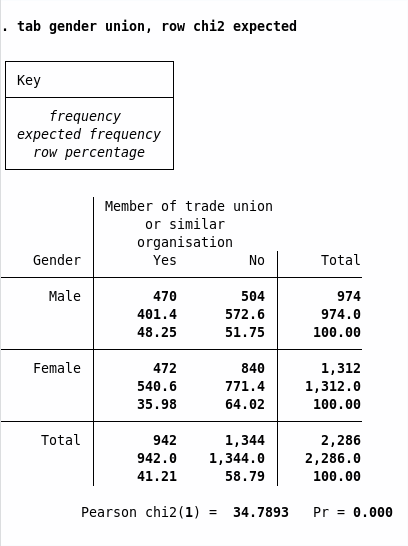
\includegraphics{../img/chi_sq_gender_union.png}}
	\caption{Cross-tabulation of gender and union membership.}
\end{figure}

\noindent\fbox{%
	\parbox{\textwidth}{%
		\begin{center}
			\textbf{How does the chi-squared test work? (In simple words)}
		\end{center}
		
		Pearson's chi-squared test applies to categorical data, and it evaluates how likely it is that an observed distribution of data is due to chance. Sometimes it is also called ``goodness of fit'' statistic because it evaluates how well the observed distribution of data fits the expected distribution if there were no relationship between the variables. Chi-squared is used to test the likelihood that your results \textit{occurred by chance}. This is the reason why we can think of Pearson's chi-squared test as a means to test the null hypothesis that the variables are independent. The test compares the frequency of each cell with the frequency one would expect to obtain were the variables independent. The expected distribution is given by the number of observations in the table's rows and columns. 
	}%
}

\subsubsection*{Measures of association}

\textit{Measures of association} summarise, with a number, the strength of a relationship. Pearson’s chi-squared test is useful in many contexts, but it is not always the best option. A chi-squared test depends greatly on the sample size; this means that the bigger the sample, the bigger chi-squared will be (and you may potentially misinterpret a chi-squared value in big samples, thus concluding that there is a strong relationship between two variables when, in fact, it may be rather weak). To solve this issue, we have two main alternatives: the coefficient phi ($\phi$), and Cramer's V. The way these two work is by simply dividing chi-squared by the maximum value chi-squared itself can be for a given table and a given number of observations (so for a 2 by 2 table this is $N$, and to compute phi we simply calculate the square root of that division. Many people interpret phi as follows:

\begin{itemize}
	\item $0 \geq \phi \leq 0.19$ = weak.
	\item $0.2 \geq \phi \leq 0.49$ = moderate.
	\item $\phi \geq 0.5$ = strong.
\end{itemize}

One thing to keep in mind is that a chi-squared test tells us about statistical significance, whereas measures of association like phi or Cramer's V tell us about the strength of the relationship (that is why the value of phi or V does not change with the sample size). Because phi is used in 2 by 2 tables (and Cramer's V is used for bigger tables), Stata always calculates Cramer's V (you could say one is a special case of the other). To calculate Cramer's V for ``gender'' and ``union membership'' we use the the command option \texttt{V} as shown below:

\begin{lstlisting}
tabulate gender union, chi2 V
\end{lstlisting}

The result of the command above shows a phi of 0.1234 (remember that phi is for 2 by 2 tables like ours). You can see now that even though chi-squared was statistically significant, phi tells us that the relationship between ``gender'' and ``trade union membership'' is rather weak! Another thing to note is that phi might take on negative values (always from -1 to 1) and Cramer's V goes from 0 to 1.

\end{document}
